\documentclass{beamer}
\usetheme{Warsaw}
\usepackage{hyperref}
\usepackage{amsmath}
\newcommand{\argmax}{\operatornamewithlimits{argmax}}
\usefonttheme[onlymath]{serif}

\title{Clockwork RNN - ICML14}
\author{Seungwoo Yoo}
\date{\today}

\begin{document}
\frame{\titlepage}

\section[Outline]{}
\frame{\tableofcontents}

\section{Introduction}
\frame
{
	\frametitle{About the authors}
    \begin{figure}[ht]  
		\begin{center}
			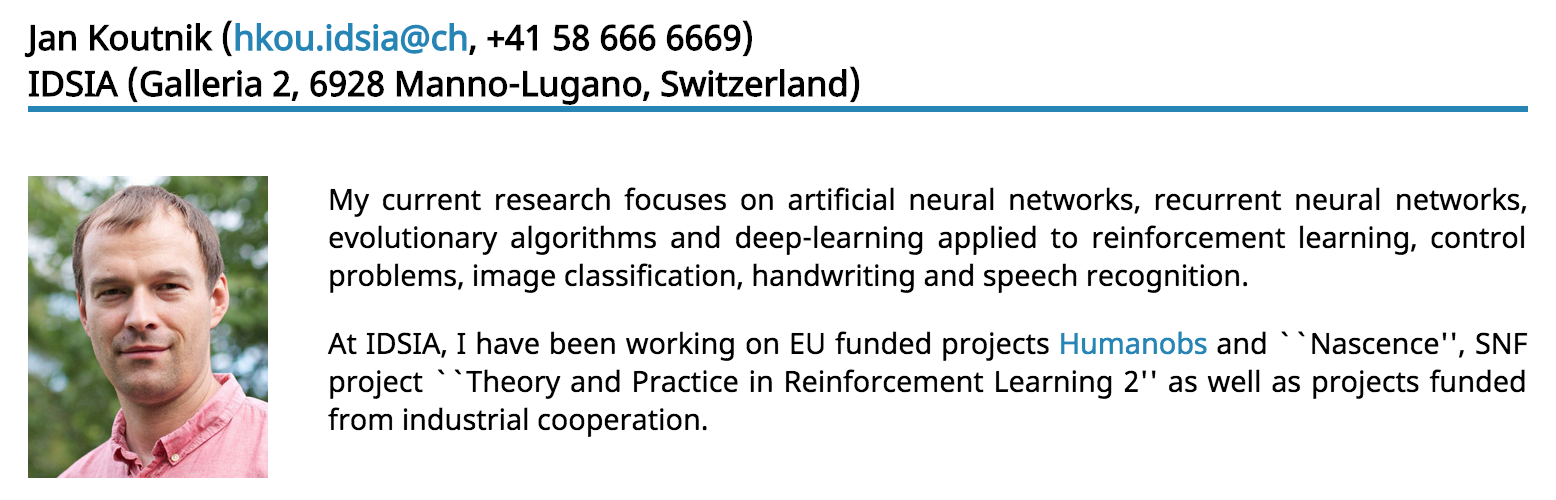
\includegraphics[width=4.1in]{Images/author.png}   
		\end{center}   
		\caption{Main author - Jan Koutnik}
	\end{figure}
}
\frame
{
	\frametitle{Contributions}
	\begin{itemize}
        \item Introduce a new RNN structure \textit{Clockwork} RNN (CW-RNN) :
			\begin{enumerate}
			\item Hidden layer is partitioned into separate module
			\item Each processing inputs at its own clock rate
			\end{enumerate}
		\item Contribution points
			\begin{itemize}
			\item CW-RNN reduces the number of RNN parameters
			\item Improve the performance and speed up the network evaluation
            \item Esp., audio signal generation and TIMIT spoken word classification
			\end{itemize}
	\end{itemize}
}
\section{Brief summary to RNN/LSTM}
\frame
{
    \frametitle{RNN summary - Forward pass}
	\begin{figure}[ht]  
		\begin{center}
			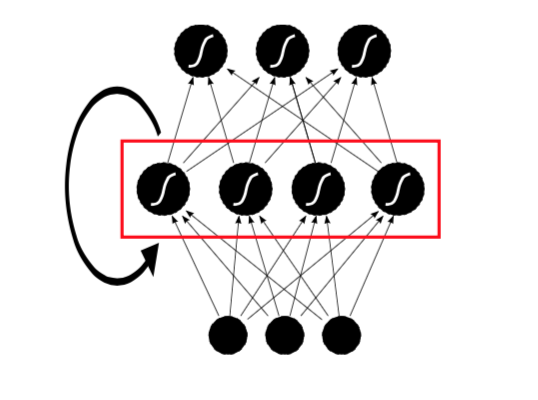
\includegraphics[width=1.6in]{Images/recurrentNN.png}   
		\end{center}   
		\caption{Illustrations of the RNN}
	\end{figure}
    \begin{itemize}
        \item Hidden units : 
        $ a_h^t = {\sum_{i=1}^I} W_{ih}x_i^t + \sum_{h'=1}^H w_{h'h} {b_{h'}}^{t-1} $ \\
        Usually initial values $b_i^0$ are chosen to zero / 
        Some cases RNN stability can be improved by using nonzero initial values.
        \item Actifaction function :
        $ b_h^t = \theta_h(a_h^t) $
        \item Output units : 
        $ a_k^t = \sum_{h=1}^H w_{hk}b_h^t $
    \end{itemize}
}
\frame
{
    \frametitle{RNN summary - Backward pass \\ Backpropagation through time (BPTT)}
    \begin{itemize}
        \item Like standard backpropagtion, consists of a repeated chain rule (depends on the next $t+1$ state) \\ 
            \vspace{0.1in}
            $ \delta_h^t = \theta'(a_h^t) \Big( \sum_{k=1}^K \delta_k^t w_{hk} + 
            \sum_{h'=1}^H \delta_{h'}^{t+1} w_{hh'} \Big)$ \\
            \vspace{0.1in}
            where $\delta_j^t \equiv \frac{\partial O}{\partial a_j^t} $
        \item Since the weights to and from each unit in the hidden layer are the same at every time step, 
            we need to sum over the whole sequence to get the derivatives : \\
            \vspace{0.1in}
            $ \frac{\partial O}{\partial w_{ij}} = \sum_{t=1}^T \frac{\partial O}{\partial a_j^t} \frac{\partial a_j^t}{\partial w_{ij}} = \sum_{t=1}^T \delta_j^t b_i^t $
    \end{itemize}
}
\frame
{
    \frametitle{BDRNN summary}
	\begin{figure}[ht]  
		\begin{center}
			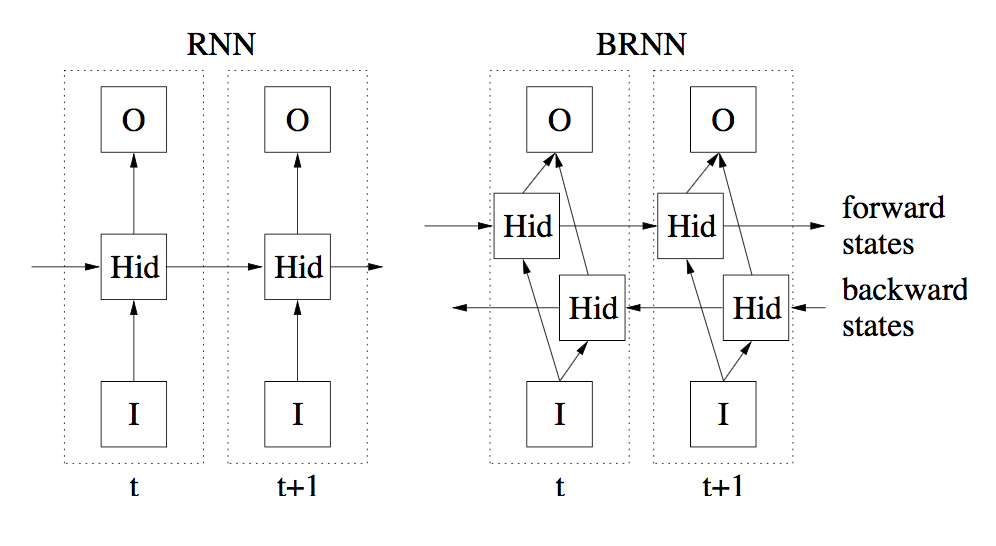
\includegraphics[width=2.2in]{Images/BDRNN_RNN.png}   
		\end{center}   
		\caption{Comparison between BDRNN and RNN}
	\end{figure}
    \begin{itemize}
        \item BDRNN (Bidirectional recurrent neural network) 
        \item Present each training sequence forwards and backwards to two seperate recurrent hidden layers, 
            both of which are connected to the same output layer
    \end{itemize}
}
\frame
{
    \begin{itemize}
        \item Forward pass for BDRNN 
            \begin{itemize} 
                \item Generally same as for a undirectional RNN, 
                \item The input sequence is presented in opposite directions to the two hidden layers. 
                \item The ouput layer is not updated until both hidden layers have processed the entire input sequence:
	            \begin{figure}[ht]  
	            	\begin{center}
	            		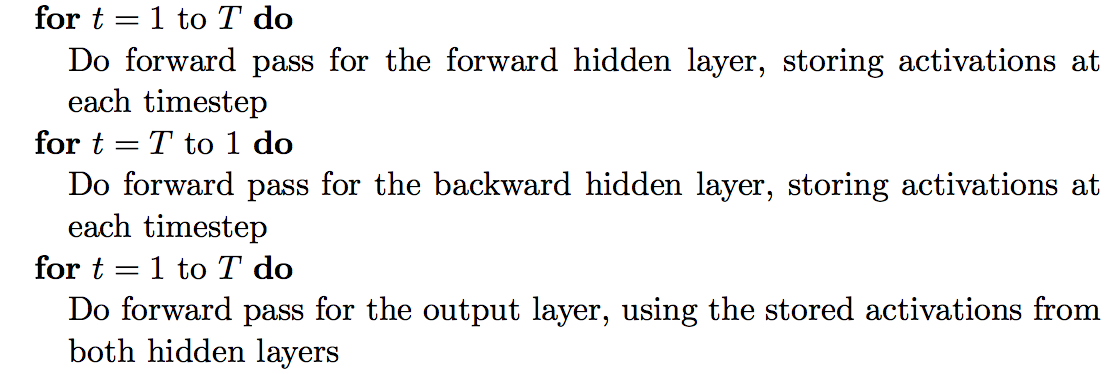
\includegraphics[width=3.5in]{Images/BDRNN_forward_pass.png}   
	            	\end{center}   
	            \end{figure}
            \end{itemize}
    \end{itemize}
}
\frame
{
    \begin{itemize}
        \item Backward pass for BDRNN 
            \begin{itemize} 
                \item Similar to the backward pass proceeds as for a standard RNN training with BPTT  
                \item All the output layer $ \delta $ terms are calculated first, 
                    then fed back to the two hidden layers in opposite directions:
	            \begin{figure}[ht]  
	            	\begin{center}
	            		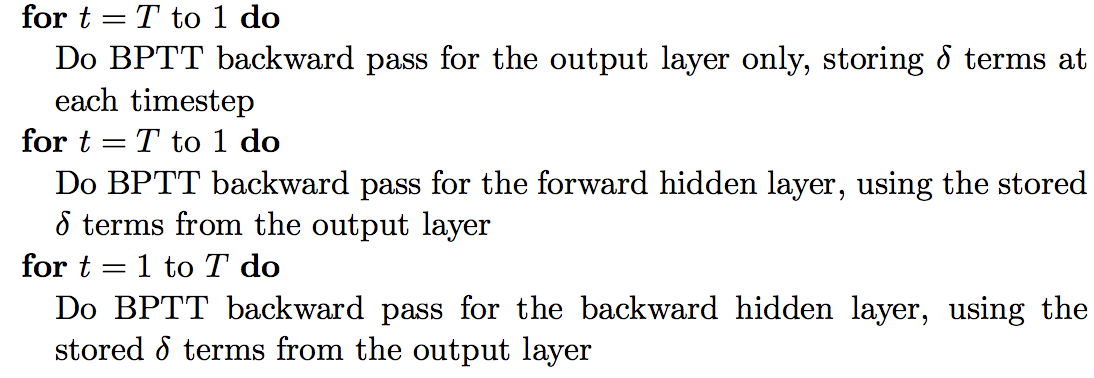
\includegraphics[width=3.5in]{Images/BDRNN_backward_pass.png}   
	            	\end{center}   
	            \end{figure}
            \end{itemize}
    \end{itemize}
}
\end{document}
